\documentclass[pdflatex,sn-mathphys-num]{sn-jnl}% Math and Physical Sciences Numbered Reference Style

\usepackage{graphicx}%
\usepackage{multirow}%
\usepackage{amsmath,amssymb,amsfonts}%
\usepackage{amsthm}%
\usepackage{mathrsfs}%
\usepackage[title]{appendix}%
\usepackage{xcolor}%
\usepackage{textcomp}%
\usepackage{manyfoot}%
\usepackage{booktabs}%
\usepackage{algorithm}%
\usepackage{algorithmicx}%
\usepackage{algpseudocode}%
\usepackage{listings}%


\begin{document}

\title[Article Title]{Politics of emotions or propaganda?}

\author{\fnm{Timur} \sur{Rezepov 34177A}}

\affil{\orgdiv{Master's Degree Course in Data Science for Economics}}
\affil{\orgdiv{Natural Language Processing course, A.Y.  2024-2025}}
\affil{\orgdiv{Prof. Alfio Ferrara}}
\affil{\orgdiv{Dott. Sergio Picascia, Dott.ssa Elisabetta Rocchetti}}


\maketitle

\section{Introduction}\label{sec1}

This project explores how emotional language is used in political texts to influence perception and manipulate audience response. The data analyzed in the project is the transcription of US 2020 Presidental Debates available on Kaggle\footnote{US 2020 Presidental Debates: \\ https://www.kaggle.com/datasets/headsortails/us-election-2020-presidential-debates}. 

Emotion classification models based on pre-trained BERT architectures have been shown to outperform other approaches (Hsu and Ku, 2018\footnote{https://doi.org/10.18653/v1/W18-3505}). To obtain emotion annotations, the DistilBERT Classifier\footnote{https://keras.io/keras_hub/api/models/distil_bert/distil_bert_text_classifier/} was fine-tuned using some techniques and methods discussed in `GoEmotions: A Dataset of Fine-Grained Emotions`\footnote{https://arxiv.org/abs/2005.00547}. 


\section{Research question and methodology}\label{sec2}

Emotional language is a powerful tool in political speeches, used to persuade, mobilize, and connect with audiences on a deeper level. For example, words evoking fear or anger create a sense of urgency, while disapproval and guilt can create negative impressions of opponent's views.

This project aims to analyze the emotional language used by Donald Trump and Joe Biden in their speeches during the 2020 U.S. Presidential Election. Precisely, each candidate uses distinct communication strategies tailored to their target audiences, seeking to evoke specific emotional responses and strengthen their position.

\subsection{Analysis methodology}

The approach used comprises of building emotional profiles: the quantitative characteristic of how often different emotions(sentiments) used in the speech.
Specifically the analysis focuses on:
\begin{itemize}
	\item emotional profile during a specific debate event;
	\item comparison of emotional profiles across different debate events;
	\item emotion flow throughout a single event;
	\item emotion distribution by topic.
\end{itemize}

\subsection{Model training}

As part of the project, an emotion classification model was developed. The model is based on the pre-trained DistilBERT architecture, fine-tuned using the GoEmotions dataset. 

The GoEmotions dataset consists of 58,000 Reddit comments, each labeled with one or more of 27 emotions or marked as Neutral, making it a multi-label classification task.
Exploratory data analysis showed that the dataset is imbalanced. To address this, severely underrepresented classes were excluded, and only those emotions relevant to political discourse were retained—resulting in a set of 19 emotion classes.
\begin{figure}[h]
	\centering
	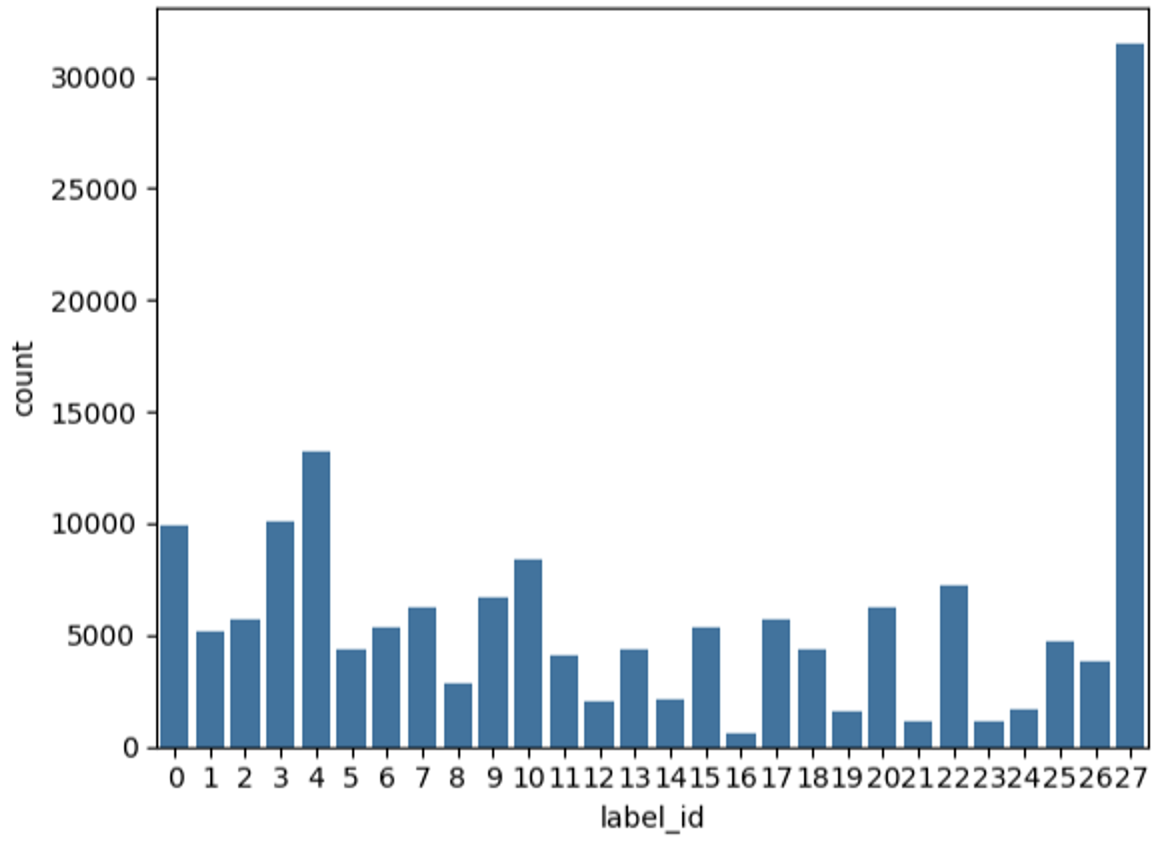
\includegraphics[width=12cm]{f1-label_distribution.png}
	\caption{Original class distribution in GoEmotions dataset}
\end{figure}

The model was compiled with the Adam optimizer (learning rate: 1e-5) and trained using the \texttt{SparseCategoricalCrossentropy} loss function and accuracy as the evaluation metric. Training was performed for 2 epochs with a batch size of 16, using a validation set to monitor performance and prevent overfitting.




\end{document}

